\documentclass{standalone}
\usepackage[svgnames]{xcolor}
\usepackage{tikz}
\usepackage[english]{babel}
\usepackage[T1]{fontenc}
\usepackage[utf8]{inputenc}
\usepackage{microtype}

\tikzstyle{peers}=[draw,circle,black]
%,bottom color=DodgerBlue, top color= white,
\tikzstyle{pose}=[color=LawnGreen]
\tikzstyle{nege}=[color=FireBrick]
\tikzstyle{c1}=[fill=DodgerBlue]
\tikzstyle{c2}=[fill=OrangeRed]
\tikzstyle{c3}=[fill=SpringGreen]
\begin{document}
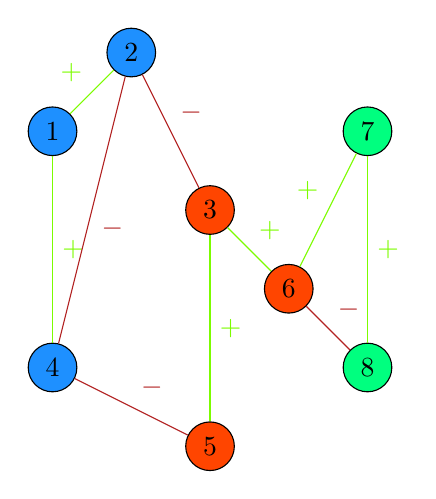
\begin{tikzpicture}[auto]
% \foreach \place/\name in
% { {(0,4)/1}, {(1,5)/2}, {(0,1)/4}, {(2,3)/3}, {(2,0)/5}, {(3,2)/6}, {(4,4)/7}, {(4,1)/8}}
%     \node[peers] (\name) at \place {\name};
\foreach \place/\name in { {(0,4)/1}, {(1,5)/2}, {(0,1)/4}}
    \node[peers,c1] (\name) at \place {\name};
\foreach \place/\name in {{(2,3)/3}, {(2,0)/5}, {(3,2)/6}}
    \node[peers,c2] (\name) at \place {\name};
\foreach \place/\name in  { {(4,4)/7}, {(4,1)/8}}
    \node[peers,c3] (\name) at \place {\name};
  \foreach \source/\dest in {1/2, 1/4, 3/5, 3/6, 6/7, 7/8}
    \draw[pose] (\source) edge node{$+$} (\dest);
  \foreach \source/\dest in {2/4,2/3,4/5,6/8}
    \draw[nege] (\source) edge node{$-$} (\dest);

\end{tikzpicture}
\end{document}

